\documentclass[a4paper]{article}

\usepackage[margin=4cm]{geometry}
\usepackage[utf8]{inputenc}
\usepackage{booktabs}
\usepackage[fleqn]{amsmath}
\usepackage{amsfonts}
\usepackage{amssymb}
\usepackage{float}
\usepackage{tikz}
\usepackage{color}
\usepackage{listings}
\usepackage{graphicx}
\usepackage{struktex}

\definecolor{mygreen}{rgb}{0,0.6,0}
\definecolor{mygray}{rgb}{0.5,0.5,0.5}
\definecolor{mymauve}{rgb}{0.58,0,0.82}
\definecolor{light-gray}{gray}{0.95}

\lstset
{
    language=C++,
    backgroundcolor=\color{light-gray},
    basicstyle=\ttfamily\linespread{1.15}\footnotesize,
    numbers=left,
    stepnumber=1,
    showstringspaces=false,
    tabsize=1,
    breaklines=true,
    breakatwhitespace=false,
    commentstyle=\color{mygreen},
    keywordstyle=\color{blue},
    stringstyle=\color{mymauve},
}

\usetikzlibrary{shapes.geometric, arrows}
\tikzstyle{box} = [rectangle, minimum width=3cm, minimum height=1cm, text centered, draw=black]
\tikzstyle{arrow} = [thin, -, >=stealth]

\graphicspath{{./IMG/}}

\title{”Programozási alapismeretek”\\ beadandó feladat:\\ ”ProgAlap beadandó” téma 1. feladat}
\date{2016-11-31}
\author{Készítette: Bárdosi Bence\\ Neptun-azonosító: VY9NJN\\ E-mail: bardosi.bence@gmail.com\\\\ Kurzuskód: IP-08PAEG\\ Gyakorlatvezető neve: Pap Gábor Sándorné}

\renewcommand*\contentsname{Tartalom}
\renewcommand*\figurename{}


\begin{document}
  \pagenumbering{gobble}
  \maketitle
  \newpage

  \pagenumbering{arabic}
  \tableofcontents
  \newpage

  \section{Felhasználói dokumentáció}
    \subsection{Feladat}
      Egy iskolában egyéni és összetett tanulmányi versenyt tartottak.
      A versenyekben összesen N tanuló vett részt. A versenyek száma M.
      Ismerjük versenyenként az induló tanulókat és elért pontszámukat.
      Az összetett versenyben csak azon tanulók eredményét értékelik,
      akik az összes egyéni versenyen indultak és elérték a versenyenként adott minimális pontszámot.
      \\
      \\ Készíts programot, amely megadja az egyéni versenyek győzteseinek rangsorát!
    \subsection{Futási környezet}
      IBM PC, exe futtatására alkalmas, 32-bites operációs rendszer (pl. Windows 10). Nem igényel egeret.
    \subsection{Használat}
      \subsubsection{A program indítása}
        A program a \textbf{.\textbackslash VY9NJN\textbackslash bin\textbackslash Release\textbackslash VY9NJN.exe} néven található a tömörített állományban. A \textbf{VY9NJN.exe} fájl kiválasztásával indítható.
      \subsubsection{A program bemenete}
        A program az adatokat a billentyűzetről olvassa be a következő sorrendben:
        \begin{table}[H]
          \centering
          \caption{Bemenet}
          \label{tab:table1}
          \begin{tabular}{ccl}
            \toprule
            \# & Adat & Magyarázat \\
            \midrule
            $1$ & $N$ & Tanulók száma $(1 \leqslant N \leqslant 100)$ \\
            $2$ & $M$ & Versenyek száma $(1 \leqslant M \leqslant 100)$ \\
            $3$ & $Min_1$ & Az 1. verseny minimum ponthatára $(0 \leqslant Min_1 \leqslant 50)$ \\
            $4$ & $Min_2$ & A 2. verseny minimum ponthatára $(0 \leqslant Min_2 \leqslant 50)$ \\
            . \\
            . \\
            . \\
            $M+2$ & $Min_M$ & Az M. verseny minimum ponthatára $(0 \leqslant Min_M \leqslant 50)$ \\
            $M+2+1$ & $Para_1$ & Az 1. verseny paraméterei (lásd: table2) \\
            $M+2+2$ & $Para_2$ & A 2. verseny paraméterei (lásd: table2) \\
            . \\
            . \\
            . \\
            $M+2+M$ & $Para_M$ & Az M. verseny paraméterei (lásd: table2) \\
            \bottomrule
          \end{tabular}
        \end{table}
        \begin{table}[H]
          \centering
          \caption{Egy adott verseny paraméterei}
          \label{tab:table2}
          \begin{tabular}{ccl}
            \toprule
            \# & Adat & Magyarázat \\
            \midrule
            $1$ & $Ind_i$ & A versenyen indulók száma $(1 \leqslant Ind_i \leqslant N)$ \\
            $2$ & $S_{i,1}$ & Az első tanuló sorszáma $(1 \leqslant S_{i,1} \leqslant N)$ \\
            $3$ & $P_{i,1}$ & Az első tanuló által elért pont $(1 \leqslant P_{i,1} \leqslant 100)$ \\
            $4$ & $S_{i,2}$ & A második tanuló sorszáma $(1 \leqslant S_{i,2} \leqslant N)$ \\
            $5$ & $P_{i,2}$ & A második tanuló által elért pont $(1 \leqslant P_{i,2} \leqslant 100)$ \\
            . \\
            . \\
            . \\
            $2*Ind_i$ & $S_{i,Ind_i}$ & Az $Ind_i$. tanuló sorszáma $(1 \leqslant S_{i,1} \leqslant N)$ \\
            $2*Ind_i+1$ & $P_{i,Ind_i}$ & Az $Ind_i$. tanuló által elért pont $(1 \leqslant P_{i,1} \leqslant 100)$ \\
            \bottomrule
          \end{tabular}
        \end{table}
      \subsubsection{A program kimenete}
        A program kiírja az egyéni versenyek győzteseinek rangsorát.
        A kimenet első sorába az egyéni győzelmet elért tanulók számát,
        amelyet a győztesek sorszáma követi, győzelmek száma szerint csökkenő,
        azon belül sorszám szerint növekvő sorrendben.
      \subsubsection{Minta bemenet és kimenet}
        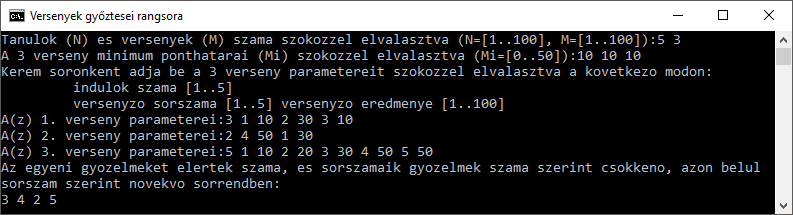
\includegraphics[width=\textwidth]{felhJo.PNG}
      \subsubsection{Hibalehetőségek}
        Az egyes bemeneti adatokat a fenti mintának megfelelően kell megadni.
        Hiba, ha a bármely bemenő adat nem egész szám, nem esik az adott intervallumba,
        vagy ha nem szám.
        Hiba esetén a program "HIBA!"-t jelez és újrakérdezi az adott adatot.
        \subparagraph{Mintafutás hibás bemeneti adatok esetén:}
        \begin{center}
          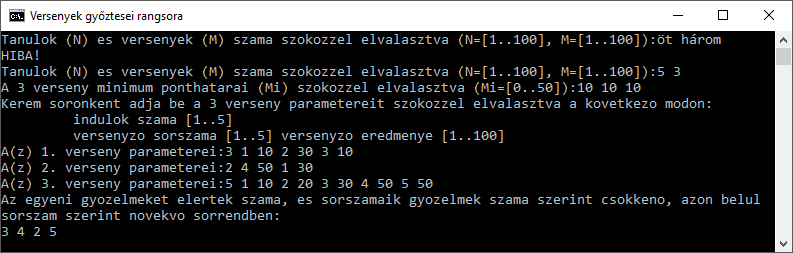
\includegraphics[width=\textwidth]{felhHibas.PNG}
        \end{center}



  \newpage

  \section{Fejlesztői dokumentáció}
    \subsection{Feladat}
    Egy iskolában egyéni és összetett tanulmányi versenyt tartottak.
    A versenyekben összesen N tanuló vett részt. A versenyek száma M.
    Ismerjük versenyenként az induló tanulókat és elért pontszámukat.
    Az összetett versenyben csak azon tanulók eredményét értékelik,
    akik az összes egyéni versenyen indultak és elérték a versenyenként adott minimális pontszámot.
    \\
    \\ Készíts programot, amely megadja az egyéni versenyek győzteseinek rangsorát!
    \subsection{Specifikáció}
    \begin{align*}
      \mathbf{Be:}\, &N \in \mathbb{N} \\
      &M \in \mathbb{N} \\
      &Min \in \mathbb{N}^M \\
      &P \in \mathbb{N}^{NxM}
    \end{align*}
    \begin{align*}
      \mathbf{Ki:}\, &T \in \mathbb{N} \\
      &Nyert \in \mathbb{N}^T
    \end{align*}
    \begin{align*}
      \mathbf{EF:}\, &N \in \left [ 1 .. 100 \right ] \\
      &M \in \left [ 1 .. 100 \right ] \\
      &\forall i \in \left [ 1 .. M \right ] : Min_i \in \left [ 0 .. 50 \right ]
    \end{align*}
    \begin{align*}
      \mathbf{UF:}\, &T=\sum_{i=1}^{N}1 \, \wedge \\
      &\quad Db(i) \geqslant 1 \\
      &Nyert \subseteq \left [ 1 .. N \right ] \, \wedge \\
      &\forall i \in \left [ 1 .. T \right ] : Db(Nyert_i) \geqslant 1 \, \wedge \\
      &\forall i \in \left[ 1 .. (T-1) \right ] : Nyert_i \, \gtrdot \, Nyert_{i+1}
    \end{align*}
    \begin{align*}
      \mathbf{Def:}\, &\quad Db(x)=\sum_{j=1}^{M}1   \\
      &P_{x,j}=Max\left(P_{\left [ 1..N \right ],j}\right) \\
      \\
      &x \, \gtrdot \, y \Leftrightarrow \left\{
                \begin{array}{ll}
                  Db(x) \neq Db(y) : Db(x) > Db(y)\\
                  Db(x) = Db(y) : x < y\\
                \end{array}
              \right. \\
      &Max(P_{X,y})=\left (k > 0\mid \exists \ i\in X: k= P_{i,y} \wedge \forall \ i \in X: k \geqslant P_{i,y} \right )
    \end{align*}
    \subsection{Fejlesztői környezet}
    IBM PC, exe futtatására alkalmas operációs rendszer (pl. Windows 10). \\
    mingw32-g++.exe c++ fordítóprogram (v4.9.2), Code::Blocks (v16.01) fejlesztői környezet.
    \subsection{Forráskód}
    A teljes fejlesztői anyag –kicsomagolás után– a \textbf{ProgAlap\_bead} nevű könyvtárban található meg.
    A fejlesztés során használt könyvtár-struktúra:
    \begin{table}[H]
      \centering
      \caption{könyvtár-struktúra}
      \label{tab:table3}
      \begin{tabular}{ll}
        \toprule
        Állomány & Magyarázat \\
        \midrule
        .\textbackslash VY9NJN\textbackslash main.cpp & C++ forráskód \\
        .\textbackslash LaTeX\textbackslash Dokumentacio.tex & Ezen dokumentáció LaTeX kódja \\
        .\textbackslash Dokumentacio.pdf & Ez a fájl \\
        .\textbackslash minta\textbackslash & Mintabemeneteket tartalmazó könyvtár \\
        \bottomrule
      \end{tabular}
    \end{table}
    \subsection{Megoldás}
      \subsubsection{Programparaméterek}
        \subparagraph{Konstans}
        \begin{center}
        \begin{tabular}{lcl}
          MERET & : & \textbf{Egész} (100) [tanulók és versenyek maximális száma]  \\
        \end{tabular}
        \end{center}
        \subparagraph{Változó}
        \begin{center}
        \begin{tabular}{lcl}
          N & : & \textbf{Egész} \\
          M & : & \textbf{Egész} \\
          Min & : & M hosszú \textbf{vektor} \\
          P & : & NxM méretű \textbf{mátrix} \\
        \end{tabular}
        \end{center}
      \subsubsection{Programfelépítés}
        \subparagraph{A program által használt modulok (és helyük):}
        \begin{center}
        \begin{tabular}{lcl}
          main.cpp & - & program, a forráskönyvtárban \\
          iostream & - & képernyő-, és billentyűkezelés, a C++ rendszer része \\
        \end{tabular}
        \end{center}
      \subsubsection{Függvénystruktúra}
        \begin{tikzpicture}[node distance=2cm]
          \node (mego) [box] {megold};
          \node (fo) [box, above of=mego] {Főprogram};
          \node (beolv) [box, left of=mego, xshift=-2cm] {beolvas};
          \node (kiir) [box, right of=mego, xshift=2cm] {kiir};
          \node (db) [box, below of=mego] {Db};
          \node (max) [box, below of=db] {Max};
          \draw [arrow] (fo) -- (mego);
          \draw [arrow] (fo) -- (beolv);
          \draw [arrow] (fo) -- (kiir);
          \draw [arrow] (mego) -- (db);
          \draw [arrow] (db) -- (max);
        \end{tikzpicture}
      \subsubsection{Algoritmus}
        \subparagraph{Főprogram: }
        \begin{center}
          \begin{struktogramm}(69,20)[FOPROGRAM]
  \assign{\(beolvas(N,\ M,\ Min,\ P)\)}
  \assign{\(megold(N,\ M,\ T,\ Min,\ P,\ Nyert)\)}
  \assign{\(kiir(T,\ Nyert)\)}
\end{struktogramm}

        \end{center}
        \subparagraph{Alprogramok: }
        \begin{center}
          \begin{struktogramm}(131,30)[{beolvas(N[Egész],\ M[Egész],\ Min[M\ Vektor],\ P[NxM\ Mátrix])}]
  \assign{\(Be:\ N\ -\ [1..MERET]\)}
  \assign{\(Be:\ M\ -\ [1..MERET]\)}
  \assign{\(Be:\ Min[1..M]\ -\ [0..50]\)}
  \assign{\(Be:\ P[1..N][1..M]\ -\ [1..100]\)}
\end{struktogramm}

          \begin{struktogramm}(152,90)[{megold(N[Egész],\ M[Egész],\ T[Egész],\ P[NxM\ Mátrix],\ Nyert[T\ Vektor])}]
  \assign{\(T:=0\)}
  \while{\(i:=1..N\)}
   \ifthenelse{6}{6}{\(Db(i,\ N,\ M,\ P,\ db)\ >=\ 1\)}{i}{n}
    \assign{\(T:=T+1\)}
   \change
   \ifend
  \whileend
  \while{\(i:=1..N\)}
   \assign{\(Nyert[i]:=i\)}
  \whileend
  \while{\(i:=N..2\ (-1)es\acute evel\)}
   \while{\(j:=1..i\)}
    \ifthenelse{6}{6}{\(db[j]\ <\ db[j+1]\)}{i}{n}
     \assign{\(S:=db[j]\)}
     \assign{\(db[j]:=db[j+1]\)}
     \assign{\(db[j+1]:=S\)}
     \assign{\(S:=Nyert[j]\)}
     \assign{\(Nyert[j]:=Nyert[j+1]\)}
     \assign{\(Nyert[j+1]:=S\)}
    \change
    \ifend
   \whileend
  \whileend
\end{struktogramm}

          \begin{struktogramm}(143,40)[{Db(i[Egész],\ N[Egész],\ M[Egész],\ P[NxM\ Mátrix],\ db[N\ Vektor])}]
  \assign{\(s:=0\)}
  \while{\(j:=1..M\)}
   \ifthenelse{6}{6}{\(P[i][j]=Max(j,\ N,\ P)\ \acute es\ nem\ P[i][j]=0\)}{i}{n}
    \assign{\(s:=s+1\)}
   \change
   \ifend
  \whileend
  \assign{\(db[i]=s\)}
  \assign{\(Db:=s\)}
\end{struktogramm}

          \begin{struktogramm}(91,30)[{Max(j[Egész],\ N[Egész],\ P[NxM\ Mátrix])}]
  \assign{\(s:=P[1][j]\)}
  \while{\(1:=1..N\)}
   \ifthenelse{6}{6}{\(P[i][j]>s\)}{i}{n}
    \assign{\(s:=P[i][j]\)}
   \change
   \ifend
  \whileend
  \assign{\(Max:=s\)}
\end{struktogramm}

        \end{center}
      \subsubsection{A kód}
        \lstinputlisting[language=C++]{../VY9NJN/main.cpp}
    \subsection{Tesztelés}
      \subsubsection{Érvényes tesztesetek}
      \subsubsection{Érvénytelen tesztesetek}
    \subsection{Fejlesztési lehetőségek}
      \begin{itemize}
        \item Adatok - a felhasználó igénye szerint - akár fájlból is fogadása.
        \item Hibás fájl-bemenetek felismerése, és a hiba helyének (sor számának) kiírása.
        \item Többszöri futtatás megszervezése.
        \item Külső adatbázis alapján tanulók sorszámának megfeleltetése neveikkel és neveik kiírása.
      \end{itemize}


\end{document}
